The blog Why Add Q to MC \ref{whyq} explained the advantages of carefully chosen, low discrepancy sampling sites for approximating multivariate integrals, or equivalently, expectations of functions of multivariate random variables
\[
\mu:  = \int_{[0,1]^d} f(\vx) \, \dif \vx = \Ex[f(\vX)], \quad \text{where } \vX \sim \cu[0,1]^d, \qquad \mu \approx \hmu_n : = \frac 1n \sum_{i=1}^n f(\vx_i).
\]
The question of when enough samples have been taken to satisfy the specified error criterion, $\abs{\mu - \hmu_n} \le \varepsilon$, is an important one.  Stopping criteria based on Bayesian credible intervals are one good way of answering this question.

Traditionally, Bayesian credible intervals take $\Order(n^3)$ operations to construct, where $n$ is the sample size.  In contrast, computing $\hmu$ requires only $\Order(n)$ operations.  Fortuitously, there is a way to reduce the computational cost of constructing the Bayesian credible interval to $\Order(n \log (n))$ when using lattice or digital net low discrepancy samples. These Bayesian stopping criteria are implemented as \code{CubBayesLatticeG} and \code{CubBayesNetG}. This blog explains the key points.

The Bayesian approach to approximating integrals assumes that the integrand, $f:[0,1]^d \to \reals$, is drawn from a Gaussian stochastic process parameterized by a (constant) mean and a covariance function defined by scale and shape parameters.  This is denoted $f \sim \mathcal{GP}(m,s^2 C_{\vtheta})$, and means that 
\[
\Ex[f(\vx)] = m, \quad \cov\bigl(f(\vt),f(\vx) \bigr) = \Ex[(f(\vt) - m)(f(\vx) - m)] = s^2 C_{\vtheta}(\vt,\vx), \qquad \forall \vt, \vx \in [0,1]^d.
\]
Here, $m$, $s$, and $C_\vtheta$, must be specified and/or estimated.  Furthermore, the multivariate integral, $\mu$, has a Gaussian distribution.  Automatic Bayesian cubature uses these assumptions to increase $n$ until we reach
$
\Prob_f  [\abs{ \mu - \hmu_n} \le \varepsilon ] \ge 99\%.
$












% First, we briefly introduce the necessary background. 
Assume the integrand, $f$, is an instance of a stochastic Gaussian process, i.e., $f \sim \mathcal{GP}(m,s^2 C_{\vtheta})$.  Specifically, $f$ is a real-valued random function with constant mean $m$ and covariance function $s^2C_{\vtheta}$, where $s$ is a positive scale factor, and $C_{\vtheta}: [0,1]^d \times [0,1]^d \to \mathbb{R} $ is a symmetric, positive-definite function and, parameterized by $\vtheta$:
\begin{multline} \label{FJH:eq:CondPosDef}
\mC_{\vtheta}^T = \mC_{\vtheta},  \quad {\va^T} \mC_{\vtheta} {\va} > 0, \quad \text{where }  \mC_{\vtheta} = \left(  C_{\vtheta}({\vx}_i,{\vx}_j)  \right)_{i,j=1}^n, \\
\text{for all } {\va} \ne 0, \;
n\in \mathbb{N}, \; \text{distinct} \; \mX = ({\vx}_1, \ldots, {\vx}_n)^T \in [0,1]^d.
\end{multline}

Automatic Bayesian cubature, $\hmu: L^1[0,1]^d \times (0,\infty) \to \reals$, approximately estimates the integral, $\mu = \int_{[0,1]^d} f(\vx) \, \dif \vx$ within user defined error tolerance, $\varepsilon$, 
 such that 
\[
{\Prob_f  [ }\abs{ \mu - \hmu(f,\varepsilon)} \le \varepsilon 
{ ] \ge 99\%} \qquad \forall \varepsilon > 0.
\]

As shown in \cite{RatHic19a}, a credible interval for the integral is given in terms of the nodes, $\{\vx_i\}_{i=1}^n$, and the covariance kernel, $C_{\vtheta}$,  by 
\begin{subequations} \label{eqn_prob_confidence_interval}
\begin{gather}
\mathbb{P}_f \left[
|\mu-\hmu| \leq \text{err}_\CI
\right] = 99\%, \\
{\text{err}_{\text{CI}}} = 2.58 \; s \; \sqrt{c_{0,{\vtheta}} - {\vc_{\vtheta}}^T \mC_{\vtheta}^{-1}\vc_{\vtheta}}
\end{gather}
\end{subequations}
where
\begin{subequations} \label{eqn:fGaussDist}
\begin{gather}
\label{eqn:fGaussDist_c0}
	c_{0,{\vtheta}} := \int_{[0,1]^{d} \times [0,1]^{d}} C_{\vtheta} (\vx,\vt) \, \dif{\vx} \, \dif{\vt}, \\
	\label{eqn:fGaussDist_vc}
 \vc_{\vtheta} := \left(  \int_{[0,1]^d} C_{\vtheta} (\vt,\vx_i) \, \dif{\vt} \right)_{i=1}^n.
	\end{gather}
\end{subequations}
where, $2.58$ represents $99\%$ quantile, which can be replaced by other quantiles and credible levels.  The formula for $\hmu$ in terms of the function values at the nodes. % is given below in Section \ref{sec:hyperparameters}.

The credible interval in \eqref{eqn_prob_confidence_interval} suggests how our automatic Bayesian cubature proceeds.  Integrand data is accumulated until the width of the credible interval, $\text{err}_{\text{CI}}$, is no greater than the error tolerance.  


As we see in the example below, computational cost increases quickly as the $n$ required to meet the error tolerance increases.  
% This motivates the fast Bayesian cubature algorithm presented in Chapter~\ref{sec:fast_BC}.







\paragraph{Example with the Mat\'ern Kernel} \label{MVN_example}

Next we demonstrate automatic Bayesian cubature using a Mat\'ern kernel as covariance kernel:
\begin{align}
\label{eqn:matern_kernel}
C_{\theta}(\vx, \vt) = \prod_{\ell=1}^d \exp(-\theta|\vx_\ell-\vt_\ell|)(1+\theta |\vx_\ell-\vt_\ell|).
\end{align}
Estimating \emph{multivariate Gaussian probabilities} on a given interval can be formulated as an integration:
% Consider the integration problem of evaluating  \emph{multivariate Gaussian probabilities}:
\begin{equation}
\label{eqn:GaussDef}
\mu = \int_{(\va,\vb)} \frac{\exp\bigl(- \frac 12 \vt^T \mSigma^{-1} \vt \bigr)}{\sqrt{(2 \pi)^d \det(\mSigma)}} \, \dvt,
\end{equation}
where $(\va,\vb)$ is a finite, semi-infinite or infinite box in $\reals^d$.  This integral does not have an analytic expression for general $\mSigma$, so cubatures are required.  

Genz \cite{Gen93} introduced a variable transformation to transform \eqref{eqn:GaussDef} into an integral on the unit cube.  Not only does this variable transformation accommodate domains that are (semi-)infinite, it also tends to smooth out the integrand better, which expedites the numerical integration.  
\iffalse
Let $\mSigma= \mL \mL^T$ be the Cholesky decomposition where $\mL = (l_{jk})_{j,k=1}^d$ is a lower triangular matrix.  Iteratively define
\begin{align*}
\alpha_1 = \Phi(a_1), 
&\qquad
\beta_1 = \Phi(b_1),
\\
\alpha_\ell(x_1,...,x_{\ell-1}) &= 
\Phi
\left(
\frac{1}{l_{\ell \ell}} 
\left(
a_\ell - \sum_{k=1}^{\ell-1} l_{\ell k} \Phi^{-1}(\alpha_k + x_k(\beta_k-\alpha_k))
\right)
\right), \quad \ell=2,...,d,
\\
\beta_\ell(x_1,...,x_{\ell-1}) &= 
\Phi
\left(
\frac{1}{l_{\ell\ell}} 
\left(
b_\ell - \sum_{k=1}^{\ell-1} l_{\ell k} \Phi^{-1}(\alpha_k + x_k(\beta_k-\alpha_k))
\right)
\right), \quad \ell=2,...,d,
\end{align*}

\fi

\begin{align}
\label{eqn:fGenzdef}
f_{\text{Genz}}(\vx) = \prod_{\ell=1}^d [\beta_\ell(\vx) - \alpha_\ell(\vx)].
\end{align}
where $\Phi$ is the cumulative standard normal distribution function.
Then, $$\mu = \int_{[0,1]^{d-1}} f_{\text{Genz}}(\vx) \, \dif{\vx}.$$
This approach transforms a $d'$ dimensional integral into a $d=d'-1$ dimensional integral.

\begin{figure}
	% \captionsetup[subfigure]{labelformat=empty}
	%\begin{subfigure}[h]{0.48\linewidth}
	%	\includegraphics[width=1.1\linewidth]{Plotting_gaussian}
	%\end{subfigure}
	\centering
	%\begin{subfigure}[h]{0.48\linewidth}
		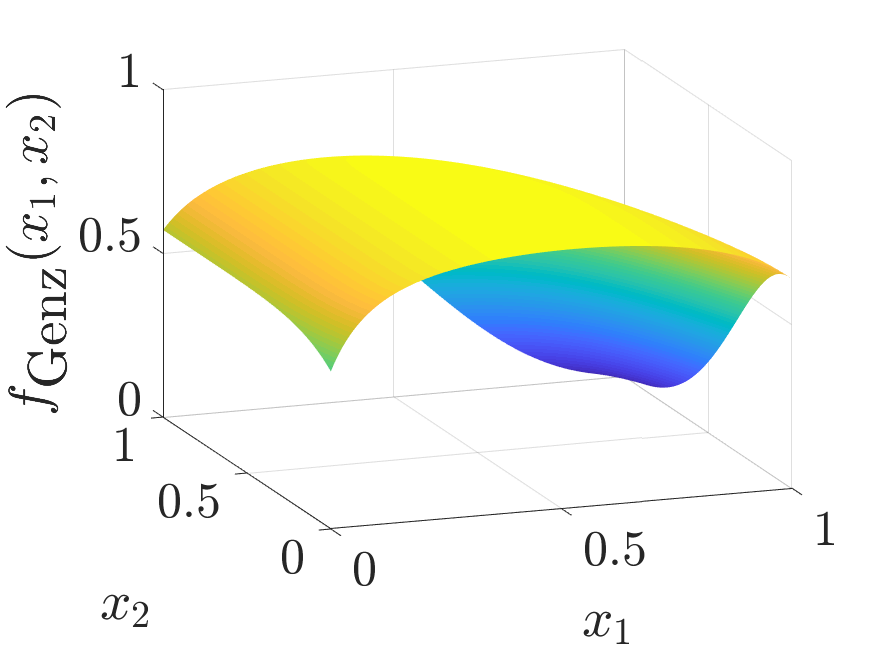
\includegraphics[width=0.75\linewidth]{BayesCub/figures/GenzFunc_varTx_none.png}
	%\end{subfigure}
	\caption{The $d=3$ multivariate normal probability transformed to an integral of $f_{\text{Genz}}$ with  $d=2$. This plot can be reproduced using \code{IntegrandPlots.m} in GAIL.}
	\label{fig:MVN_Genz}
\end{figure}

We use the following parameter values in the simulation: 
\begin{equation*}
d = 3, \quad \va = \begin{pmatrix}%[1]
-6 \\ -2 \\ -2
\end{pmatrix}, \quad 
\vb = \begin{pmatrix}%[1]
5 \\ 2 \\ 1
\end{pmatrix} , \quad 
\mL = \begin{pmatrix}%[1]
4 & 1 & 1 \\ 0 & 1 & 0.5 \\ 0 & 0 & 0.25
\end{pmatrix}.
\end{equation*}



\begin{figure}[ht]
	\centering
	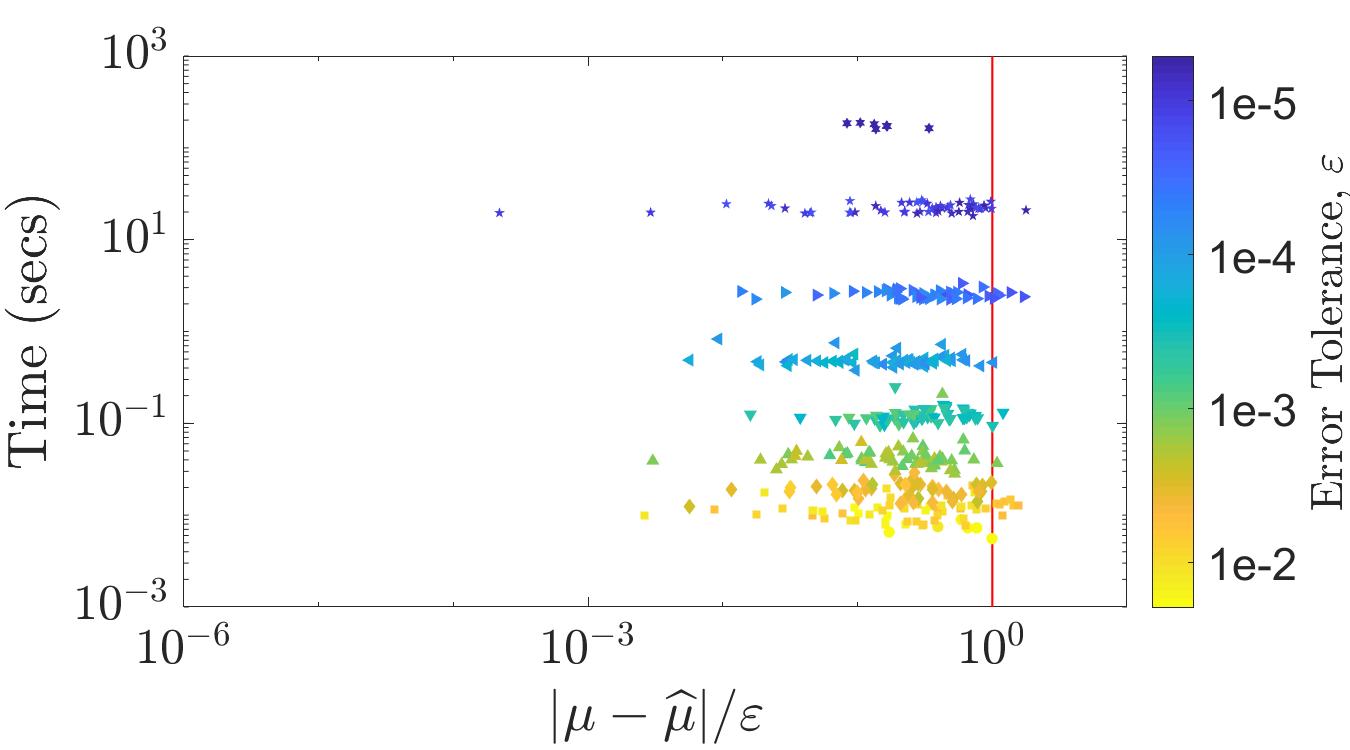
\includegraphics[width=0.9\linewidth]{BayesCub/figures/MVN_guaranteed_time_Matern_d2_2019-Jun-29}
	\caption{Multivariate Gaussian probability: Guaranteed integration using Mat\'ern kernel in $d=2$ using empirical Bayes stopping criterion within error tolerance $\varepsilon$. This figure can be conditionally reproduced using \code{matern\_guaranteed\_plots.m} in GAIL.}
	\label{fig:MVN_Metern_d2b2}
\end{figure}
\begin{figure}[ht]
	\centering
	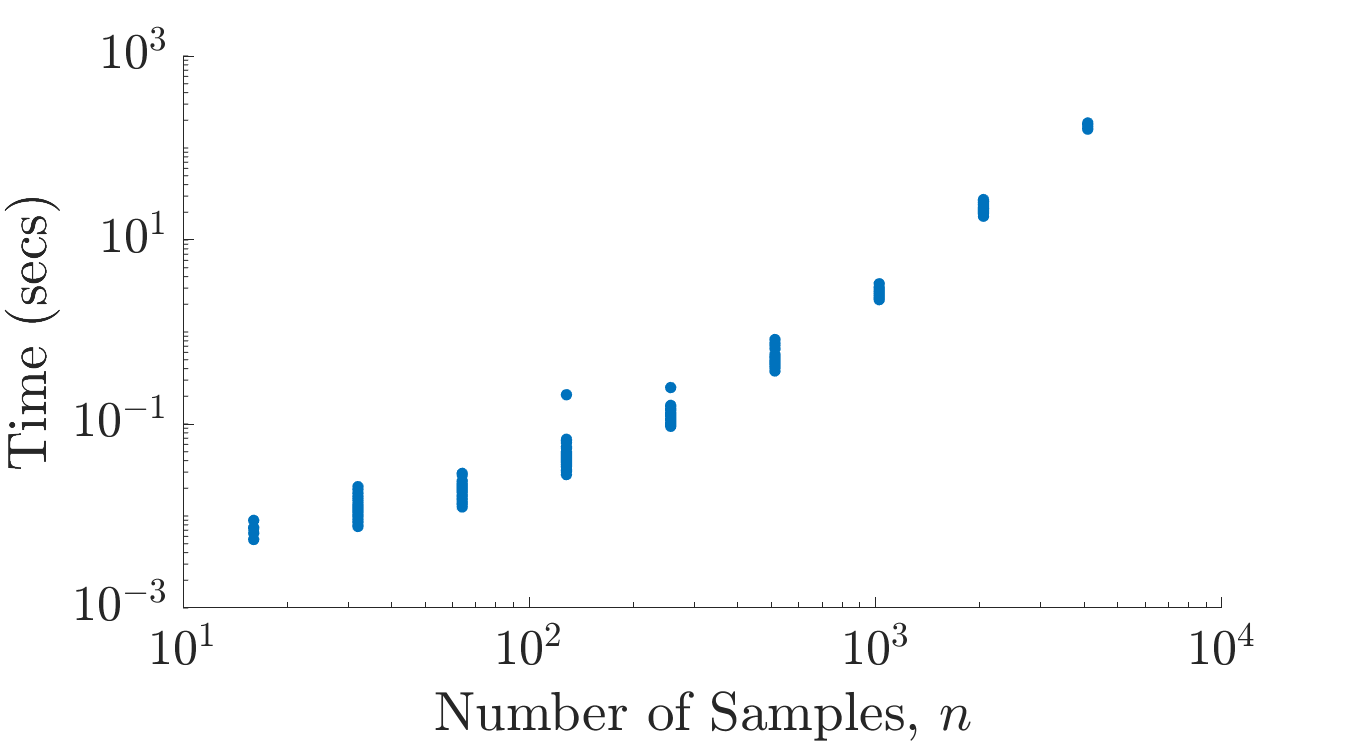
\includegraphics[width=0.9\linewidth]{BayesCub/figures/MVN_rapid_n_vs_time_Matern_d2_2019-Jun-29}
	\caption{Multivariate Gaussian probability estimated using Mat\'ern kernel in $d=2$ using empirical Bayes stopping criterion. Computation time rapidly increases with increase of $n$. This figure can be conditionally reproduced using \code{matern\_guaranteed\_plots.m} in GAIL.}
	\label{fig:MVN_Metern_d2b2_time_growth}
\end{figure}
The node sets are randomly scrambled Sobol' points \cite{DicEtal14a,DicPil10a}.  The results are for 400 randomly chosen $\varepsilon$ in the interval $[10^{-5}, 10^{-2}]$ as shown in Figure \ref{fig:MVN_Metern_d2b2}. In each run, the nodes are randomly scrambled.  We  observe the algorithm meets the error criterion 95\% of the time even though we used 99\% credible intervals.
One possible explanation is that the matrix inversions in the algorithm are ill-conditioned leading to numerical inaccuracies.  Another possible explanation is that this Mat\'ern covariance kernel is not a good match for the integrand.

%with Intel i7 3630QM and 16GB RAM memory
On our test computer, it took more than an hour to compute $\hmu_n$ with $n=2^{14}$. 
As shown in Figure \ref{fig:MVN_Metern_d2b2_time_growth}, the computation time increases rapidly with $n$. 
The empirical Bayes estimation of $\vtheta$, which requires repeated evaluation of the objective function, is the most time consuming of all. This is due to fact that the objective function needs to be computed multiple times in every iteration to find its minimum. It takes tens of seconds to compute $\hmu_n$ with $\varepsilon = 10^{-5}$.   
% In contrast, this example in Chapter~\ref{sec:NumExp} take less than a hundredth of a second to compute $\hmu_n$ with the same $\varepsilon$ using our new algorithm. Not only is the Bayesian cubature with the Mat\'ern kernel slow, but also $\mC_\vtheta$ becomes highly ill-conditioned as $n$ increases.
So, Algorithm~\ref{algorithm1} in its current form is impractical when $n$ must be large.


As $n$ increases, one expects $c_{0,\vtheta} - {\vc_\vtheta}^T{\mC_\vtheta}^{-1}{\vc_\vtheta}$ to decrease for well-chosen nodes, $\{\vx_i\}_{i=1}^n$. 
But these computations are Ill-conditioned and numerical cost of vector-matrix calculations is $O (n^3)$. This motivates us to pursue the techniques to pursue \emph{Fast Bayesian Transforms} which helps with these problems.







% \hyperlink{kappaDeriv}{\beamergotobutton{details}}.

